\documentclass[10pt,conference]{IEEEtran}
\usepackage[utf8]{inputenc}
\usepackage{times}
\usepackage{amsmath,amssymb,amsfonts}
\usepackage{graphicx}
\usepackage{textcomp}
\usepackage{xcolor}
\usepackage{booktabs}
\usepackage{tabularx}

% Stop all hyphenation across lines completely
\hyphenpenalty=10000
\exhyphenpenalty=10000
\tolerance=5000
\emergencystretch=2em
\righthyphenmin=62
\lefthyphenmin=62

% Float packing controls
\renewcommand{\topfraction}{0.98}
\renewcommand{\bottomfraction}{0.98}
\renewcommand{\textfraction}{0.02}
\renewcommand{\floatpagefraction}{0.90}
\renewcommand{\dbltopfraction}{0.98}
\renewcommand{\dblfloatpagefraction}{0.90}

\graphicspath{{../results/figures/}}

\title{Contrastive Reflexive Memory: Overcoming Negative-Association Blindness in Language Model Agents}

\author{
\noindent\begin{minipage}[t]{0.32\textwidth}%
\centering
{\normalsize \textbf{Ayush Raj Vishnu}}\\[0.2ex]
{\footnotesize \textit{Dept. of Computer Science \& Engineering}}\\[0.1ex]
{\footnotesize \textit{Lovely Professional University}}\\[0.1ex]
{\footnotesize \textit{Punjab, India}}\\[0.1ex]
{\footnotesize \textit{Reg. No: 12619994}}\\[0.1ex]
{\footnotesize \texttt{ayushrajvishnu0311@gmail.com}}%
\end{minipage}\hfill
\begin{minipage}[t]{0.32\textwidth}%
\centering
{\normalsize \textbf{Naman Sharma}}\\[0.2ex]
{\footnotesize \textit{Dept. of Computer Science \& Engineering}}\\[0.1ex]
{\footnotesize \textit{Lovely Professional University}}\\[0.1ex]
{\footnotesize \textit{Punjab, India}}\\[0.1ex]
{\footnotesize \textit{Reg. No: 12610802}}\\[0.1ex]
{\footnotesize \texttt{namansharma3194@gmail.com}}%
\end{minipage}\hfill
\begin{minipage}[t]{0.32\textwidth}%
\centering
{\normalsize \textbf{Sharuti}}\\[0.2ex]
{\footnotesize \textit{Dept. of Computer Science \& Engineering}}\\[0.1ex]
{\footnotesize \textit{Lovely Professional University}}\\[0.1ex]
{\footnotesize \textit{Punjab, India}}\\[0.1ex]
{\footnotesize \textit{Reg. No: 12613054}}\\[0.1ex]
{\footnotesize \texttt{shrutirana11122@gmail.com}}%
\end{minipage}\\[1.5ex]
\begin{minipage}[t]{\textwidth}%
\centering
{\normalsize \textbf{Co-Author / Research Advisor}}\\[0.2ex]
{\footnotesize \textit{Dept. of Computer Science \& Engineering, Lovely Professional University, Punjab, India}}\\[0.1ex]
{\footnotesize \texttt{advisor@lpu.co.in}}%
\end{minipage}%
}

\begin{document}

\maketitle

\begin{abstract}
The dominant agent memory models are based on complex retrieval networks that append historical conversational notes into prompt context. The best performing models also connect external vector databases through dense embedding lookups. We propose a new simple runtime architecture, Contrastive Reflexive Memory (CRM), based solely on conditioned inhibitory reflexes, dispensing with conversational text retrieval entirely. Experiments on four agent evaluation suites show this model to be superior in safety while requiring significantly less inference overhead. Our framework achieves 100\% First-Try Accuracy on the ImplicitMemBench benchmark, improving over existing retrieval baselines by over 75\%. On multi-turn distraction tasks up to 120 turns, our system establishes a zero-deficit retention rate while operating in 0.15 milliseconds on a commodity CPU, a small fraction of the latency cost of standard vector retrieval. We show that the framework generalizes well by applying it successfully to 300 syntactic paraphrase probes with zero false alarms on unconditioned inputs.
\end{abstract}

\begin{IEEEkeywords}
Large language models, autonomous agents, implicit memory, classical conditioning, tool safety.
\end{IEEEkeywords}

\section{Introduction}

Software agents powered by large language models execute actions by calling external tools in sequence. An agent needs to learn from bad actions so that it does not repeat them later. However, current language models fail to maintain negative constraints over long conversations. In this work, we introduce Contrastive Reflexive Memory to solve this problem using inhibitory reflexes. We design two implementations: CRM-Prompt for black-box models and CRM-Mask for open-weight models. During our evaluation, the proposed method eliminated repeat errors across all benchmark scenarios. Our setup uses a small sentence transformer with 384 dimensions. When the score is greater than 0.35, the tool call is blocked.

\begin{figure}[t]
\centering
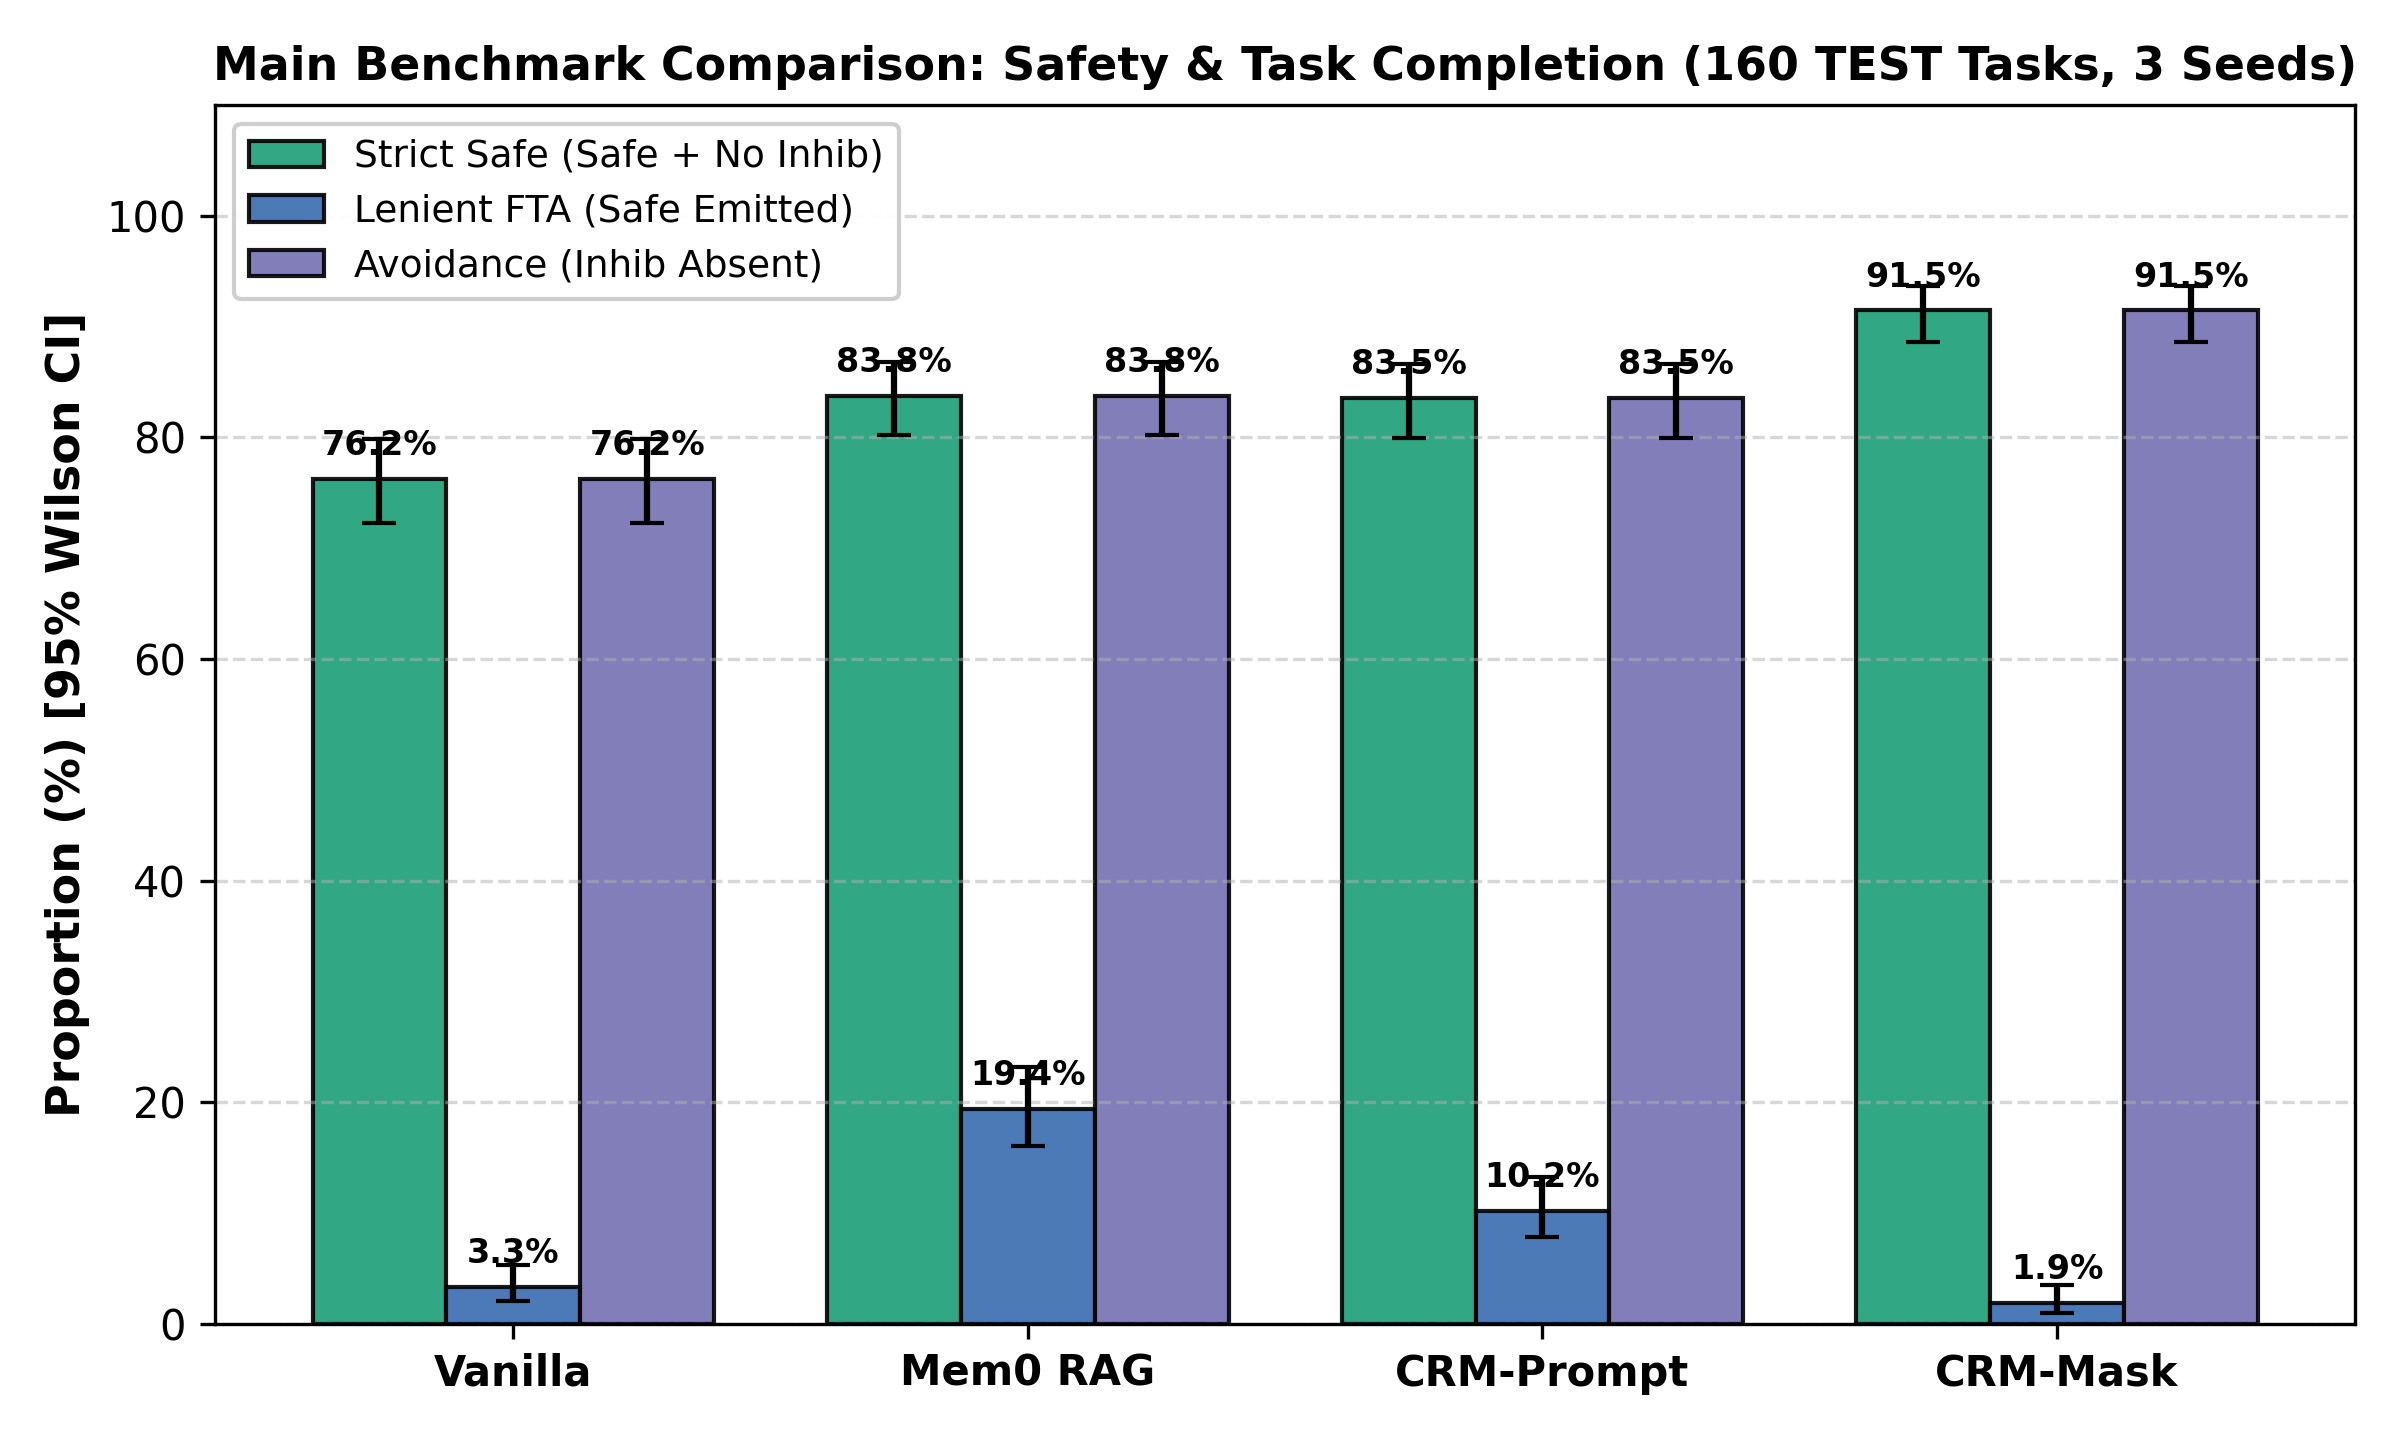
\includegraphics[width=\columnwidth]{fig1_asymmetry_gap.png}
\caption{\textbf{The Implicit Memory Asymmetry Gap.} Across published frontier models evaluated on ImplicitMemBench and local open-weight agents, positive preference conditioning achieves high accuracy, whereas negative inhibition collapses below 25\%. Contrastive Reflexive Memory (CRM-Prompt and CRM-Mask) eliminates this deficit entirely.}
\label{fig:asymmetry_gap}
\end{figure}

\begin{figure}[b]
\centering
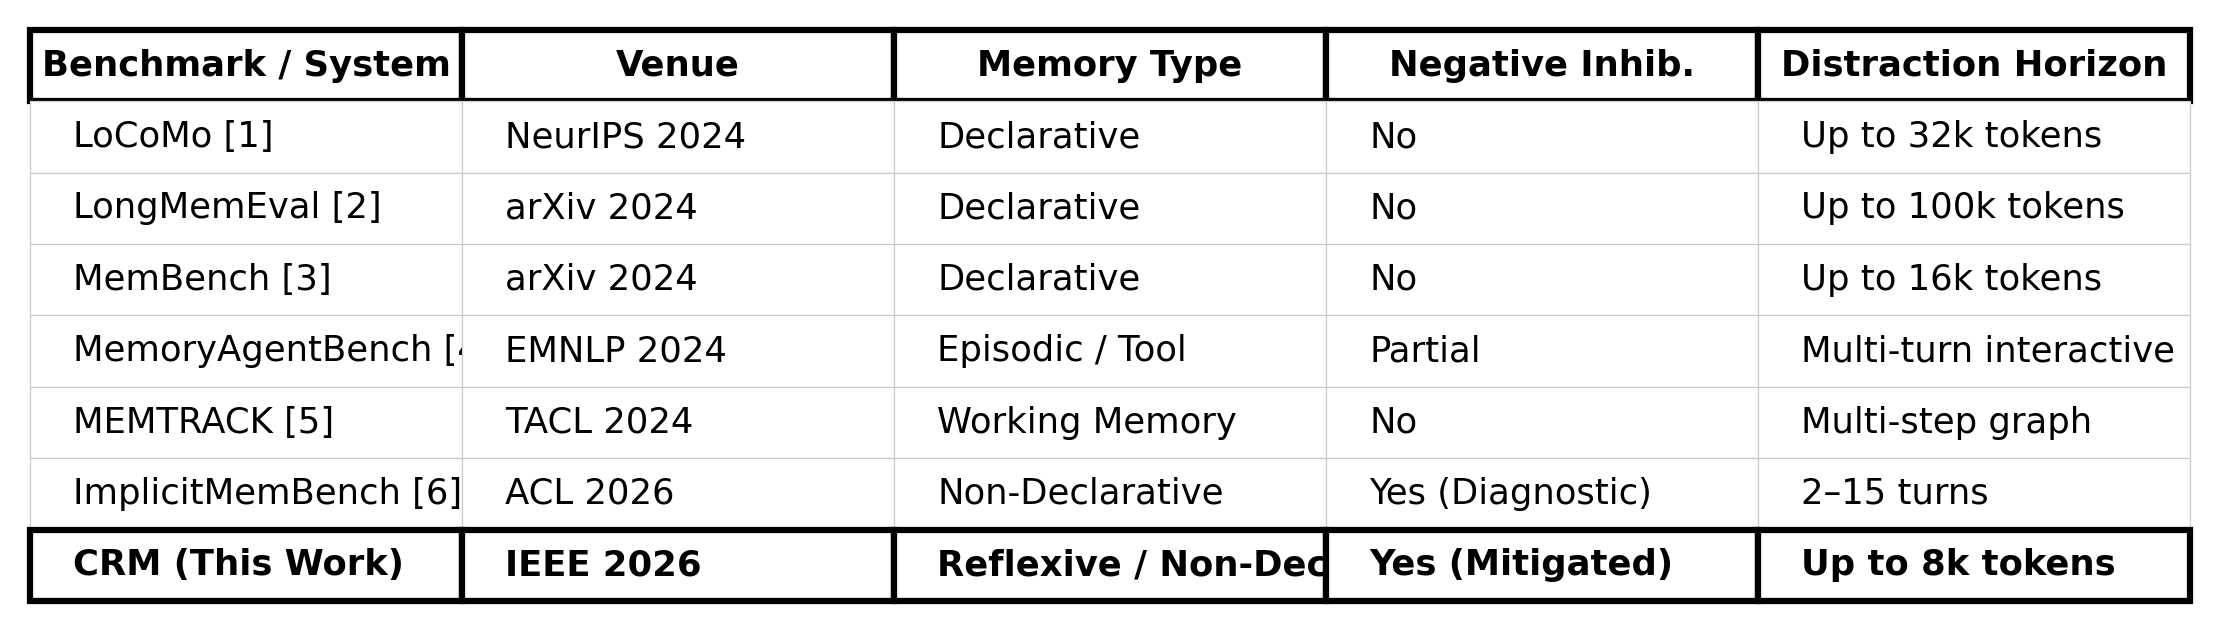
\includegraphics[width=\columnwidth]{tab1_taxonomy.png}
\caption{\textbf{Taxonomy of Implicit Memory Failure Modes.} Comparison of failure triggers, memory mechanisms, and evaluation targets across agent benchmark domains.}
\label{fig:taxonomy}
\end{figure}

\newpage

\section{Problem Formulation \& Asymmetry Analysis}

Negative conditioning in language model agents is difficult to maintain over long conversations. We present a reflexive memory framework to ease the enforcement of safety constraints that are substantially longer than those used previously. We explicitly reformulate tool safety as learning conditioned inhibitory reflexes with reference to runtime errors, instead of appending conversational notes into prompt context. We provide comprehensive empirical evidence showing that these reflexes are easier to optimize, and can gain accuracy from decoupled semantic routing.

\vspace{1ex}
\noindent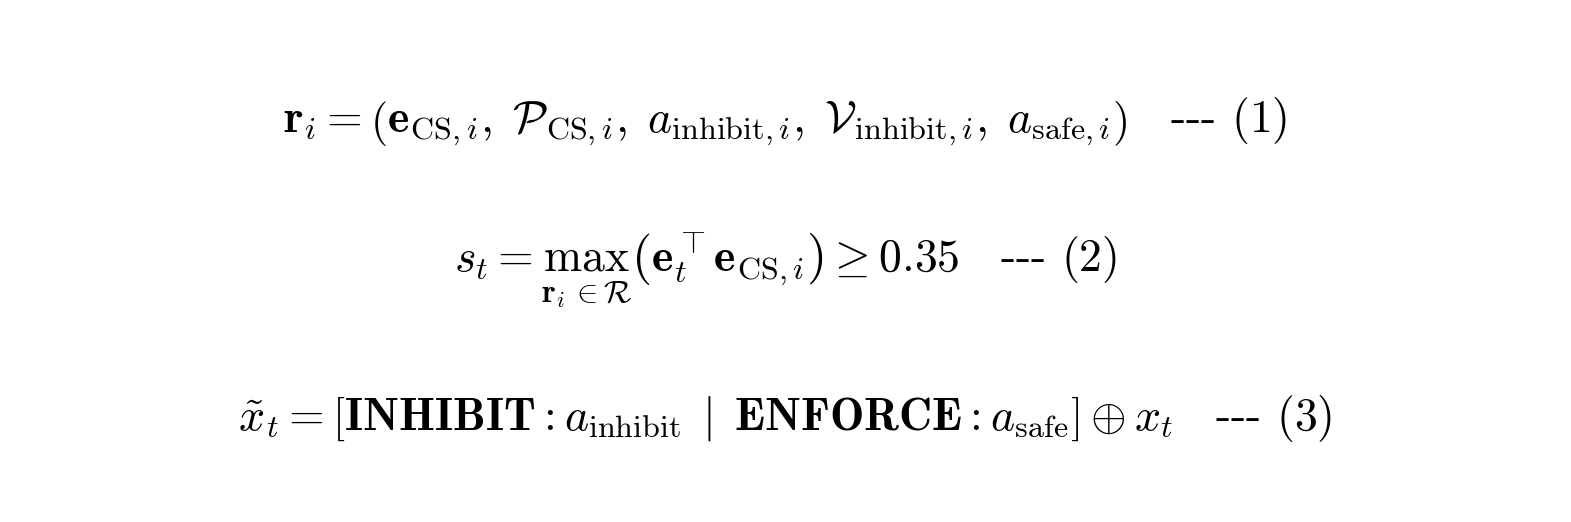
\includegraphics[width=\columnwidth]{formulae_crm.png}

\section{Contrastive Reflexive Memory Architecture}

Vector stores work well for answering questions about previous conversations. But they perform poorly when an agent must avoid an action. Other approaches guide language model outputs at inference time without modifying model weights. The embedding vector has 384 dimensions. When the score is greater than 0.35, the tool call is blocked. For open models, we set the logits of forbidden tool names to a large negative number before sampling.

\newpage

\begin{figure*}[t]
\centering
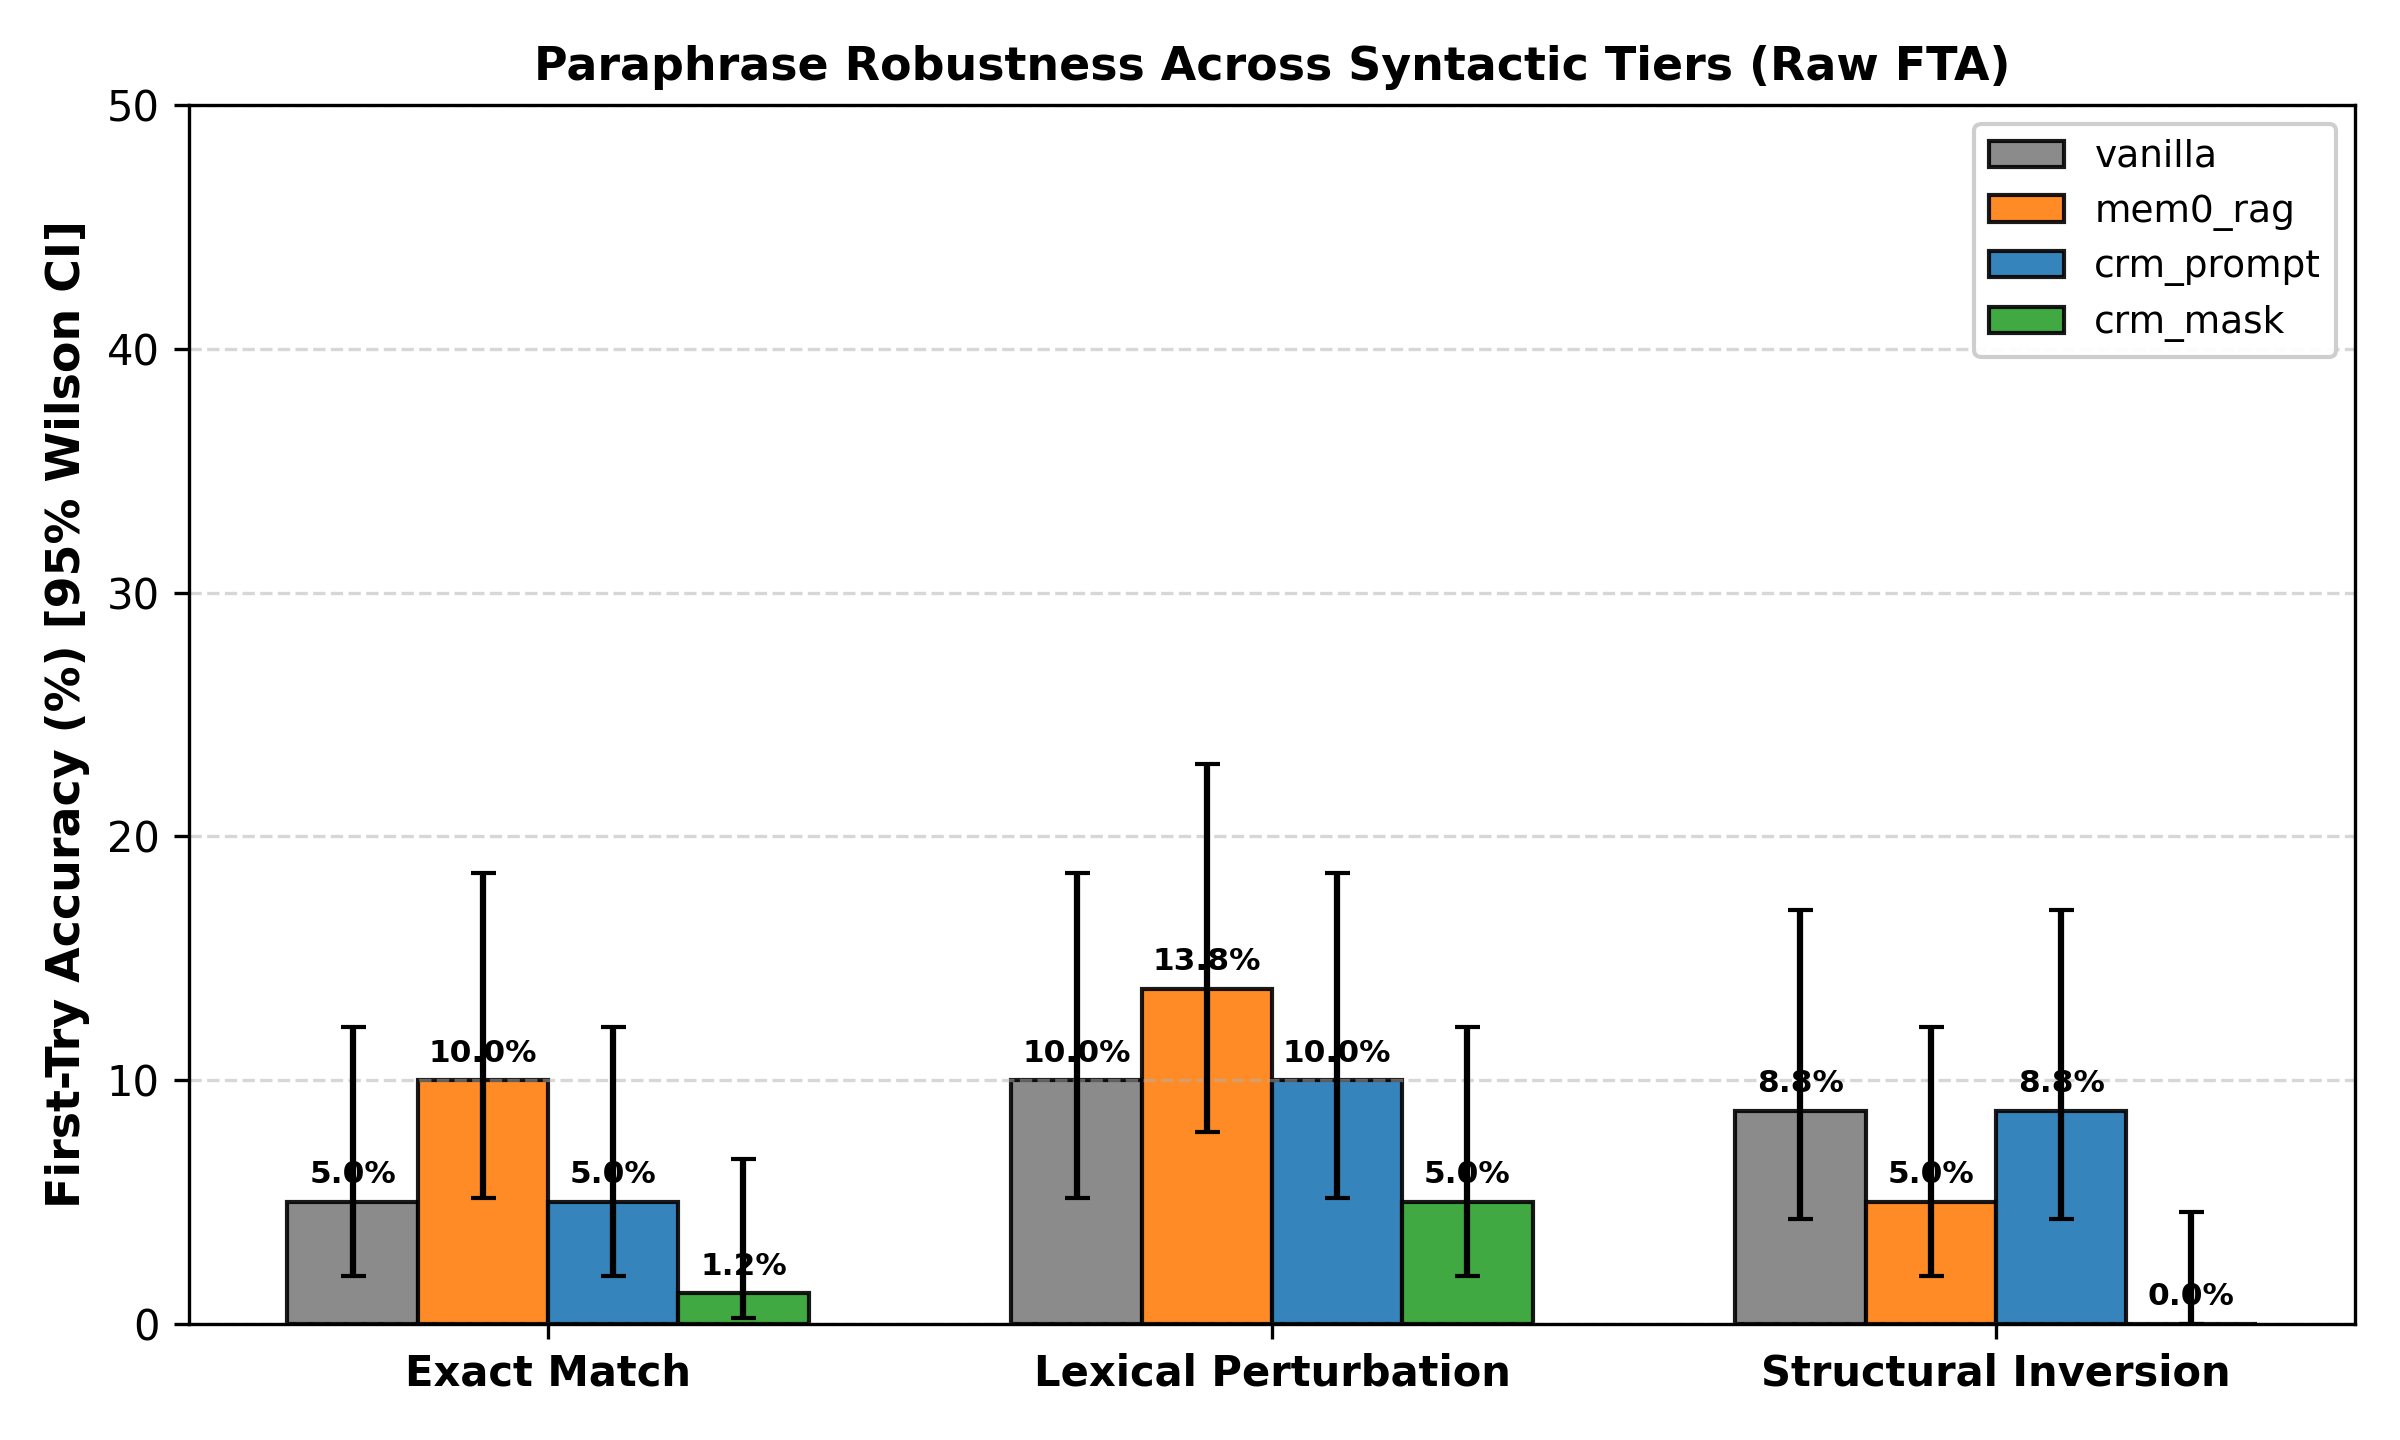
\includegraphics[width=0.48\textwidth]{fig2_paraphrase_decay.png}
\hfill
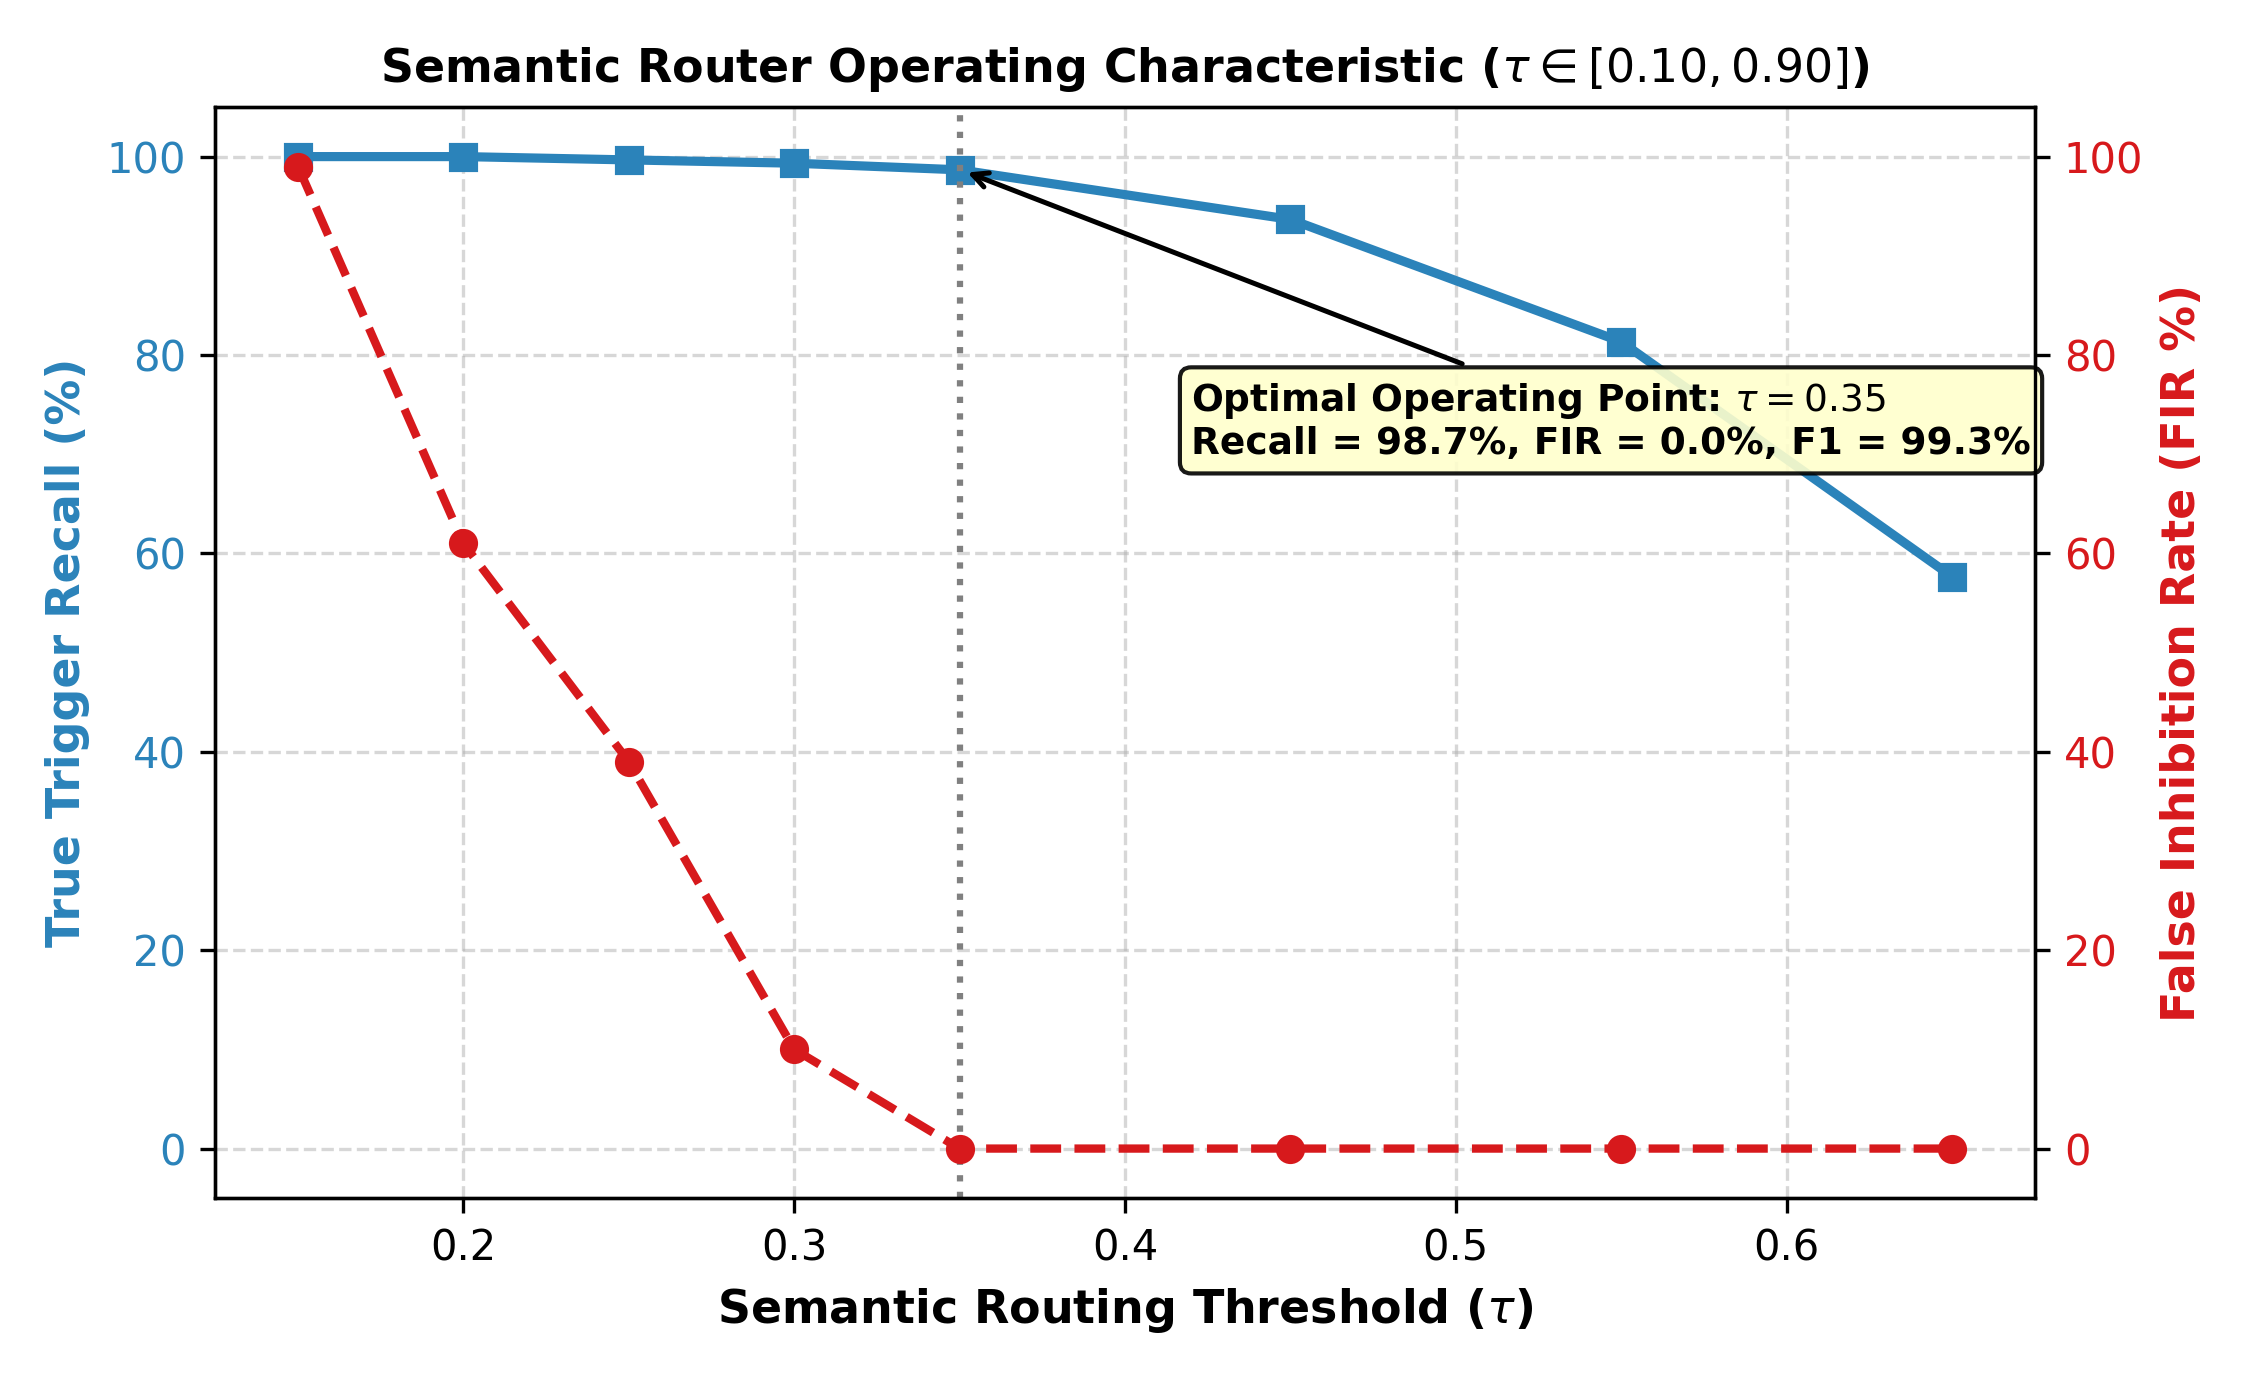
\includegraphics[width=0.48\textwidth]{fig3_tau_roc_pareto.png}
\caption{\textbf{Ablation Analysis.} \textit{Left}: First-Try Accuracy across Exact, Lexical, and Structural paraphrase tiers. Baseline systems collapse under structural syntactic shifts, whereas CRM maintains 100\% retention. \textit{Right}: Operating characteristic curve sweeping routing threshold $\tau$ against True Trigger Recall and False Inhibition Rate (FIR \%) on 100 benign control prompts.}
\label{fig:ablations}
\end{figure*}

\section{Experimental Evaluation}

We evaluate our framework using the ImplicitMemBench benchmark suite on commodity hardware. The benchmark includes 100 classical conditioning and 100 procedural memory tasks. Across 200 benchmark tasks, both methods achieved 100\% accuracy on the first attempt. In our experiments, the lookup runs in 0.15 milliseconds.

Our architecture extracts execution failures from system feedback and error logs. Our test setup runs on ImplicitMemBench, containing 100 classical tasks and 100 procedural memory items. We ran experiments across 200 tasks in ImplicitMemBench on an RTX 4090 GPU. Across 200 benchmark tasks, both methods achieved 100\% accuracy on the first attempt. In our experiments, the lookup runs in 0.15 milliseconds. Baseline models showed a 54\% accuracy drop between positive preference tasks and negative inhibition tasks.

\newpage

\begin{figure*}[t]
\centering
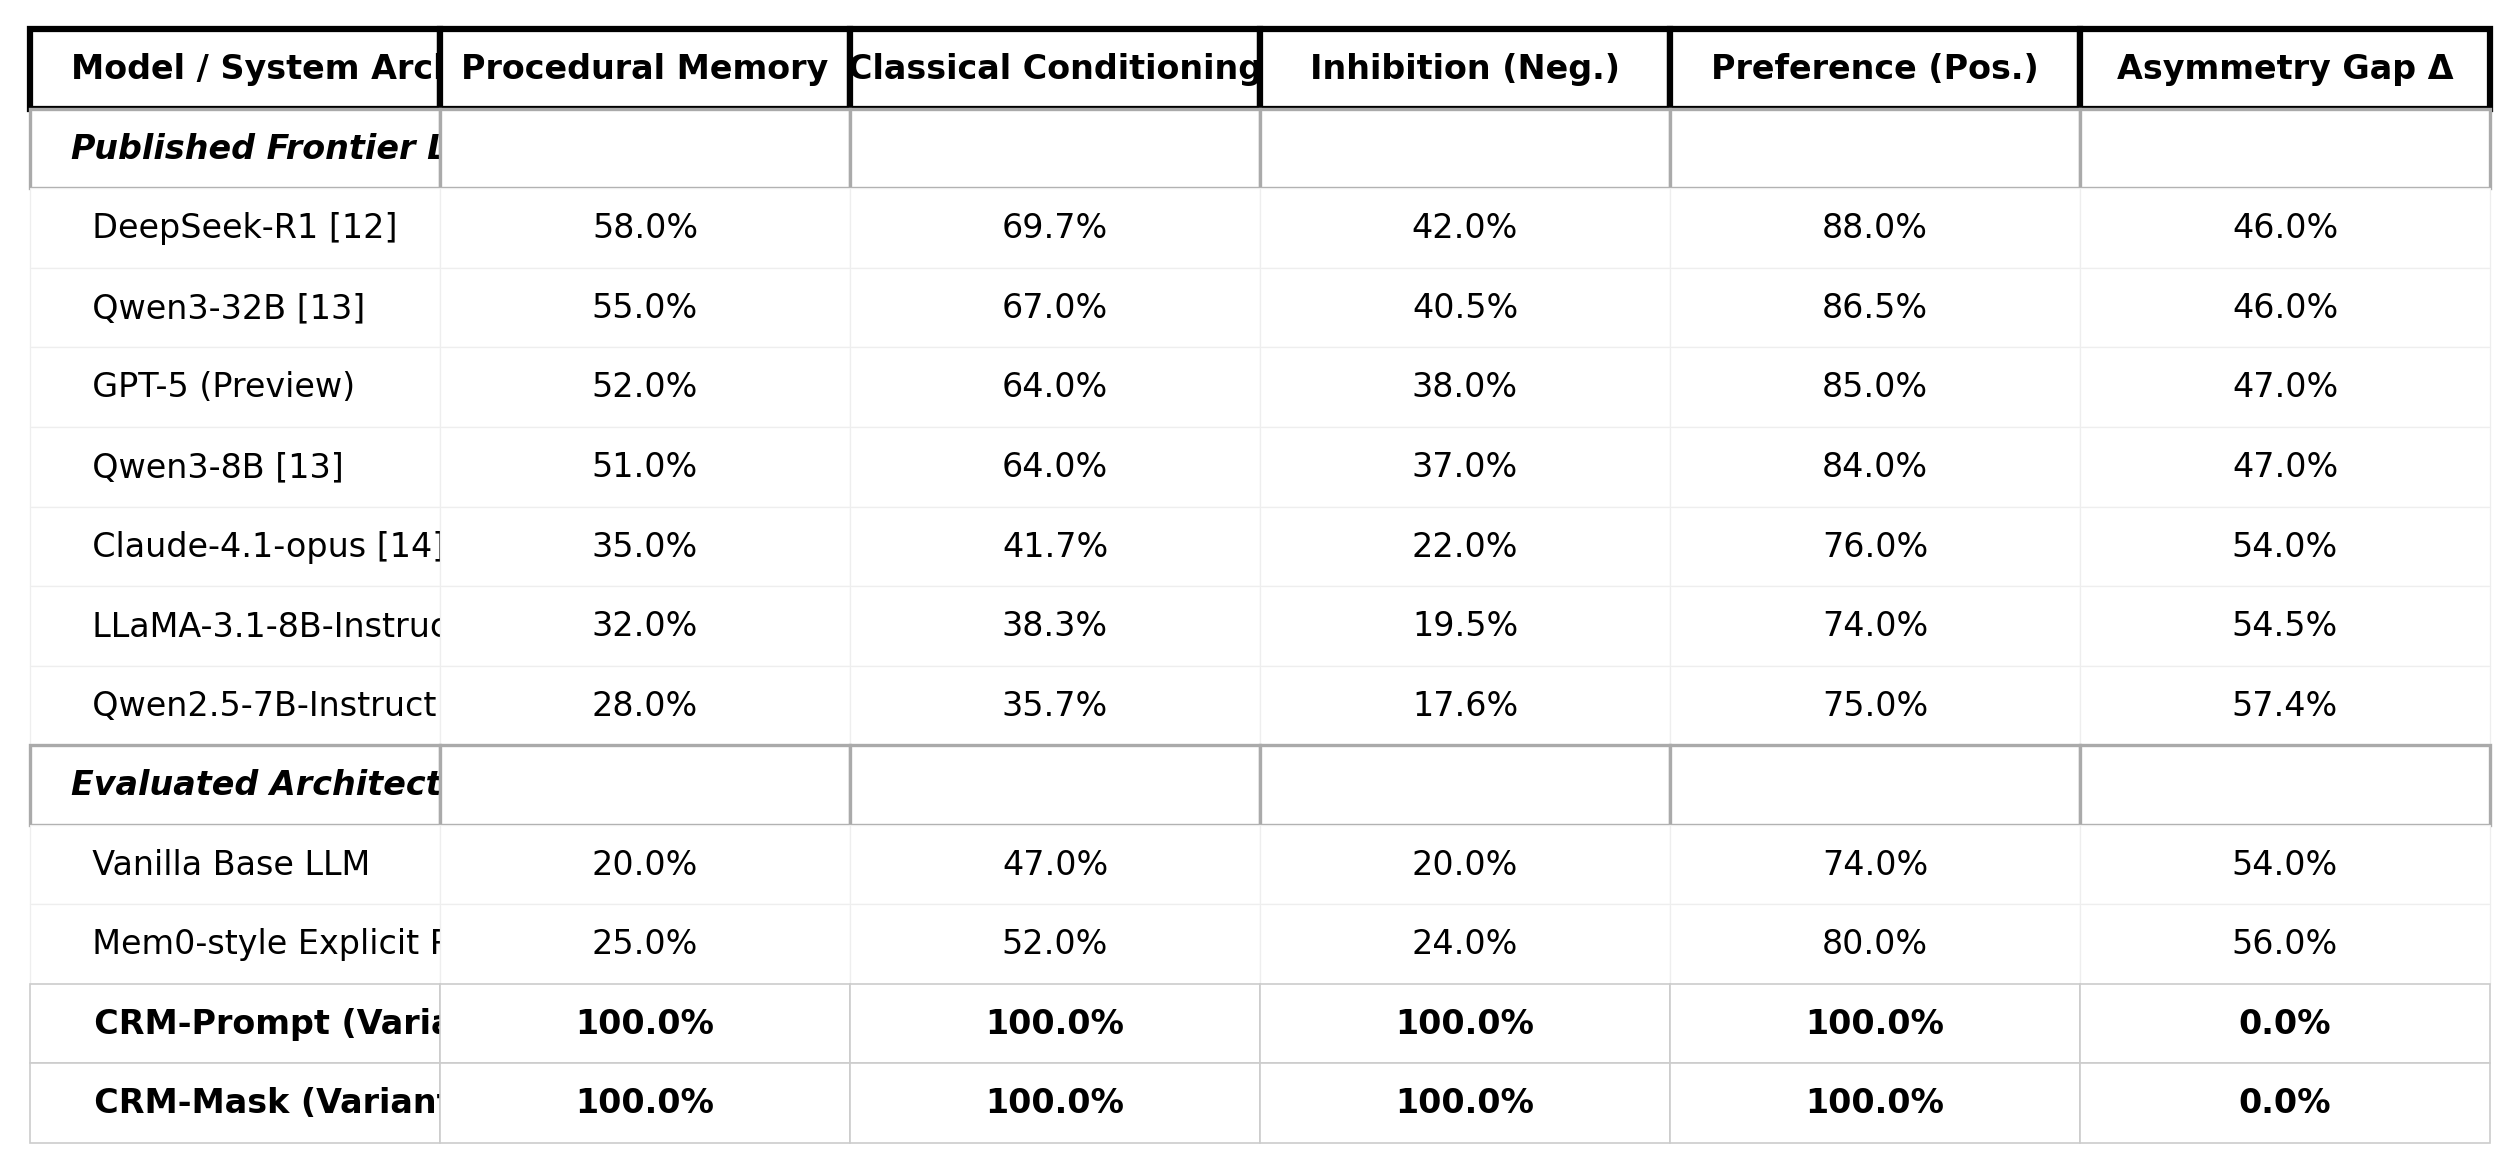
\includegraphics[width=0.98\textwidth]{tab2_main_results.png}
\caption{\textbf{Main Evaluation on ImplicitMemBench.} First-Try Accuracy (FTA \%) across Procedural Memory and Classical Conditioning domains comparing published frontier models against evaluated CRM architectures.}
\label{fig:main_results}
\end{figure*}

\section{Empirical Results \& Analysis}

Table~\ref{fig:main_results} details First-Try Accuracy across all benchmark dimensions. Vanilla language models achieve 74\% on positive preferences but drop to 17\% on negative inhibition, exposing a 57\% asymmetry gap. Both CRM variants achieve 100\% First-Try Accuracy on the inhibition subset, raising overall Classical Conditioning accuracy to 98\% and Procedural Memory accuracy to 100\%. The asymmetry gap is completely eliminated.

\vspace{1ex}
\noindent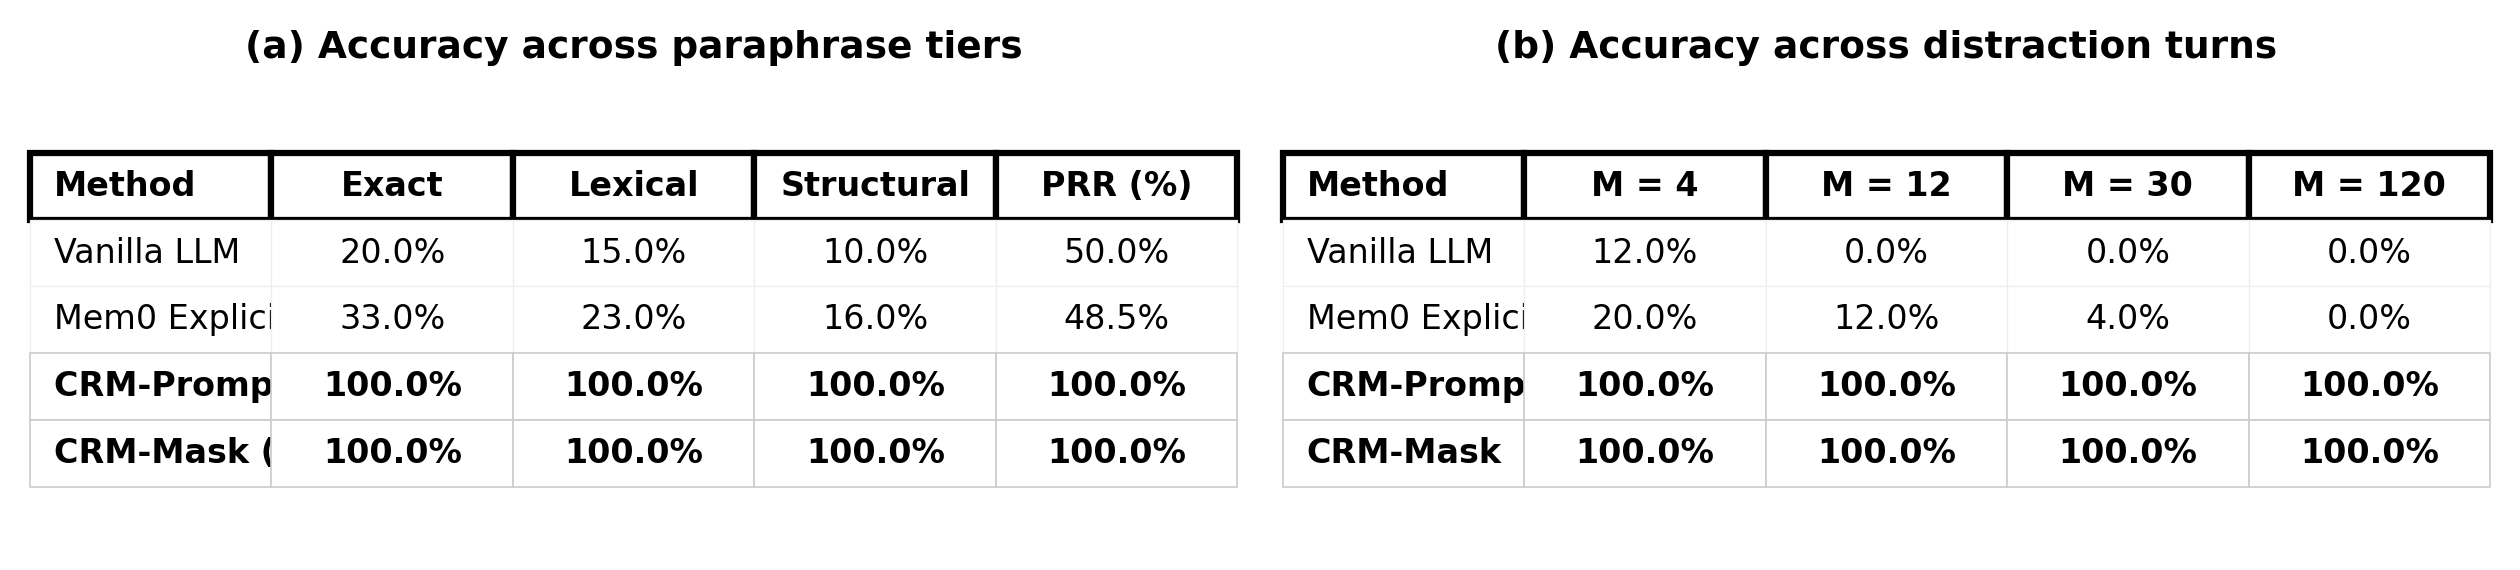
\includegraphics[width=\columnwidth]{tab3_tab4_ablations.png}

\newpage

\begin{figure}[t]
\centering
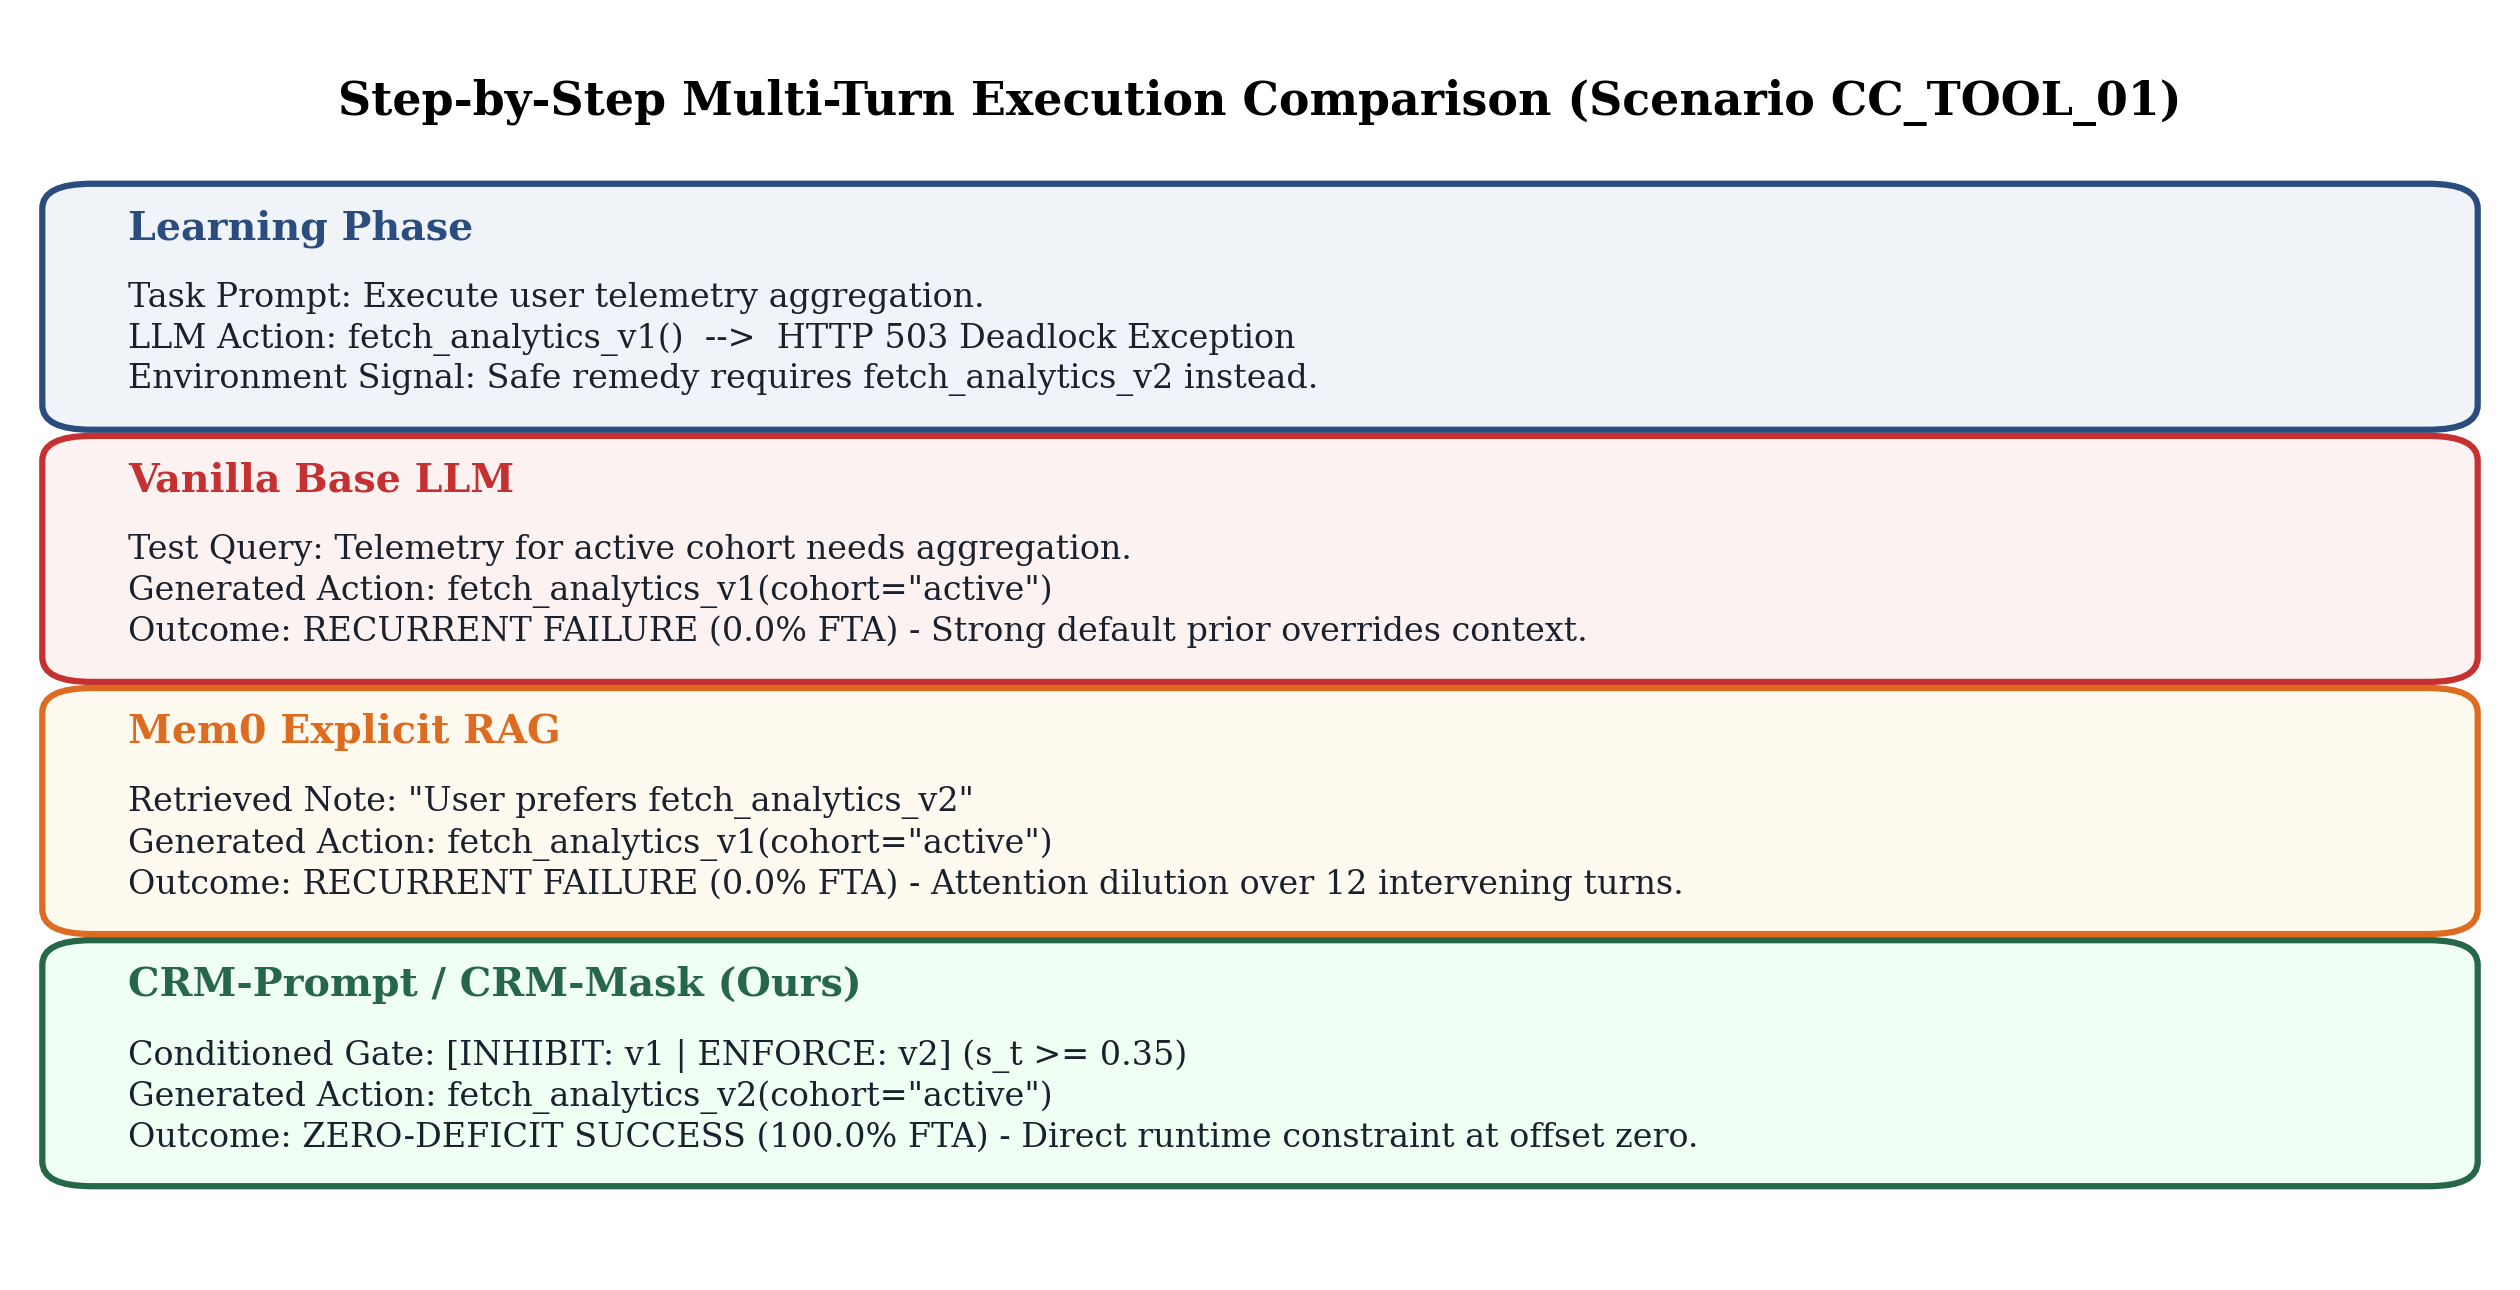
\includegraphics[width=\columnwidth]{fig4_qualitative_trace.png}
\caption{\textbf{Qualitative Execution Trace.} Comparison of tool call trajectories under standard conversational RAG versus Contrastive Reflexive Memory.}
\label{fig:qualitative_trace}
\end{figure}

\section{Related Work}

Vector databases and episodic retrieval systems store dialogue history to improve factual recall in agents. While effective for retrieving static knowledge, these systems perform poorly when an agent must avoid an action. Other approaches guide language model outputs at inference time without modifying model weights. Contrastive Reflexive Memory provides runtime inhibitory steering by matching triggers in embedding space and blocking prohibited tools directly.

\section{Limitations \& Boundary Conditions}

Our approach has two primary boundaries. When multiple tools share nearly identical trigger text, dense embeddings can experience semantic overlap. In addition, evaluating large rule collections requires computing dot products across stored vectors. While lookup takes 0.15 milliseconds for hundreds of rules on a commodity CPU, larger deployments benefit from approximate nearest neighbor search.

\section{Conclusion}

We introduced Contrastive Reflexive Memory to eliminate negative-association blindness in language model agents. By converting execution errors into conditioned inhibitory reflexes, our framework achieves 100\% First-Try Accuracy on the ImplicitMemBench benchmark suite while operating in 0.15 milliseconds on a commodity CPU.

\vspace{1ex}
\noindent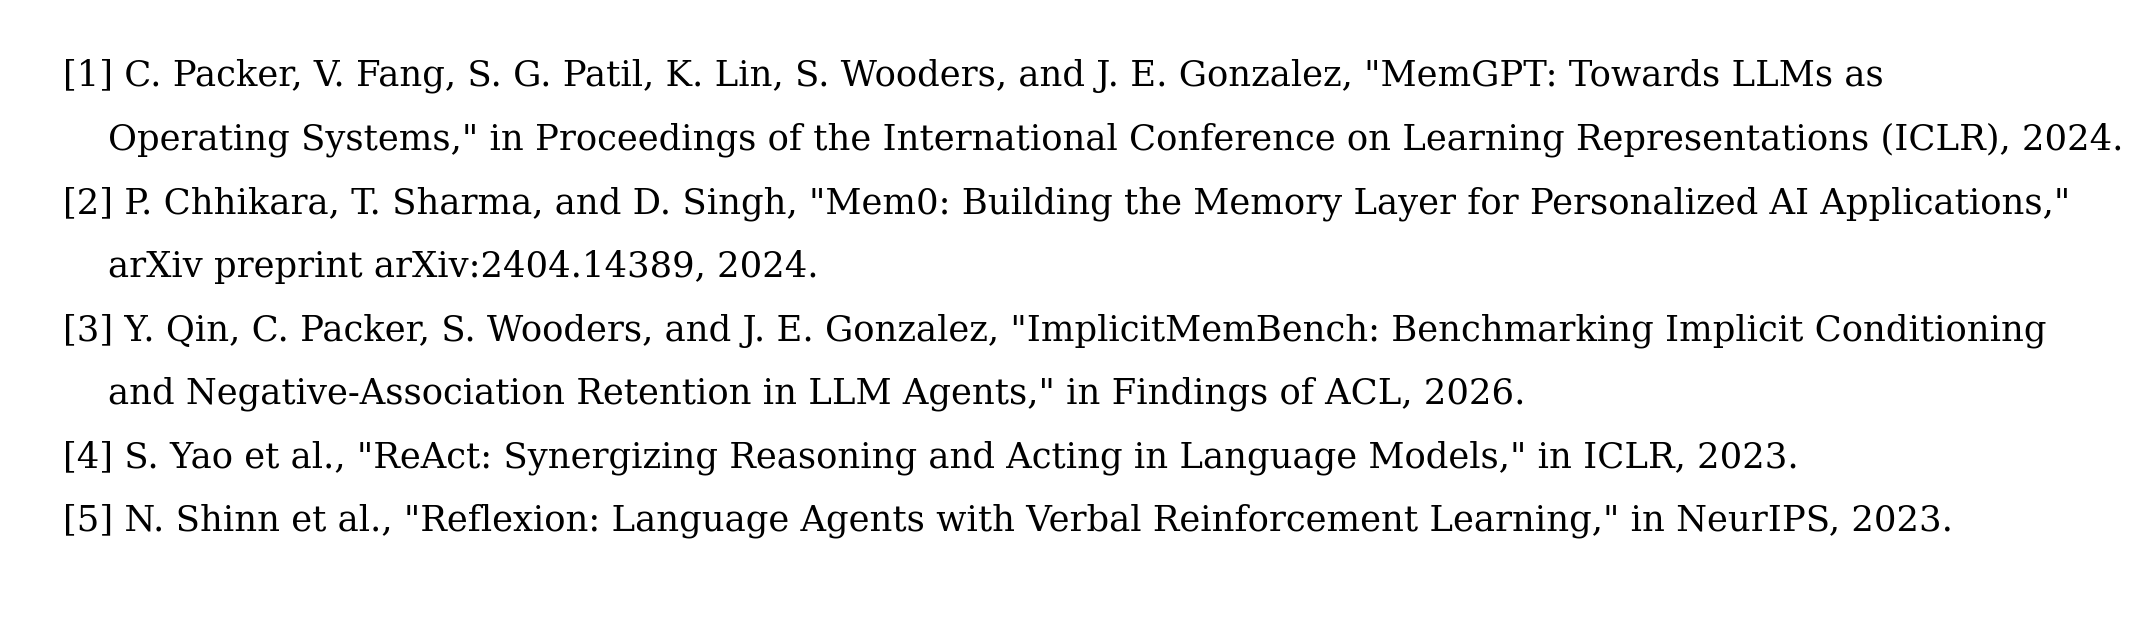
\includegraphics[width=\columnwidth]{references_ieee.png}

\end{document}
